\scanpage{137}
foncteur fibre \inserted{$\psi=\psi_{\overline k}$} sur $M'$, i.e. une section de $\mathscr G'$, d'où une \deleted{\unsure{restriction}} \deleted{\unsure{restreinte}} gerbe $\mathscr G_\psi$ de lien $G^{\unsure{\circ|0}}$, qui \deleted{\unsure{donc}} est \deleted{liée} reliée à la gerbe $\mathscr G$ de lien $G$ via $G^{\unsure{\circ|0}}\hookrightarrow G$.

\uline{NB} En général, $H^1(Q,\Gamma)\ne1$, donc il y a ici un choix \uline{très} \uuline{particulier} de trivialisation de \uline{la gerbe $\unsure{M'|M''}$}.

Considérons enfin la \deleted{gerbe} \inserted{ss-catégorie tensorielle de $M$} \inserted{$M^{(0)}$} engendrée par $M_0$ et $M'$: c'est la catégorie formée des sommes directes
\[
\sum_{i\in Z}V_i(i),
\]
où les $V_i$ sont $\in M'$, et les $V_i\in M'$ sont tous nuls sauf un nb fini
\margin{\figure{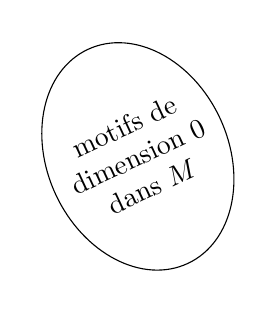
\begin{tikzpicture}\draw[rotate=25] (0,0) ellipse (1.15 and 1.5);\node[rotate=25,align=center] at (0,0) {\uline{\unsure{motifs de}}\\\uline{\unsure{dimension} $0$}\\\uline{dans $M$}};\end{tikzpicture}}}
[NB
\[
\left(\sum V_i(i)\right)\otimes\left(\sum W_j(j)\right)=\sum_n\left(\sum_{i+j=n}V_i\otimes W_j\right)(n),\qquad
\left(\sum V_i(i)\right)^\vee=\sum\check V_{\unsure{i|-i}}(-i)
\]
]
On trouve un foncteur fibre
\diagram{\begin{tikzcd}
\displaystyle\sum_{i\in Z}V_i(\unsure{k|i}) \arrow[r] & \displaystyle\sum V_i(\overline k)
\end{tikzcd}},
\margin{\diagram{\begin{tikzcd}[row sep=small,column sep=small]
M_0 & M^{(0)} \arrow[l,dash] \\
& M' \arrow[u,hook]
\end{tikzcd}}}
$\deleted{\unsure{a}}\mathscr G^{(0)}$, $\underset{\text{groupe}}{G^{(0)}}\simeq G'\times G_m$

\diagram{\begin{tikzcd}
& & \mathscr G \arrow[r] & \mathscr G^{(0)} \\
1 \arrow[r] & U \arrow[r,phantom,"\unsure{\text{—}|\longrightarrow}"] & G \arrow[r,phantom,"\unsure{\text{—}|\longrightarrow}"] & G^{(0)}=G_m\times G' \arrow[r,dash] & 1
\end{tikzcd}}
On trouve une \deleted{\unsure{restriction}} \inserted{gerbe} $\mathscr G_\chi$ sous $U$, reliée à la gerbe $\mathscr G$ sur $G$ \deleted{\unsure{par}} \unsure{et|via} $U\hookrightarrow G$.
\mspage{136}
